\section{Front End}
Elena Makarenko
\vskip 0.1in
\indent
\indent
The Methodology section describes actions that were taken and tools that were used in order to ensure that all of the project goals are achieved within the given constraints.

\subsection{Agile} 
\indent
\indent
Sometimes we underestimate the importance of planning and analysis.
Time spent on these activities might seem to be a waste of time.
Nevertheless, real-world experience shows that impact of the planning phase on project success is crucial.

\begin{figure}[ht]
    \centering
    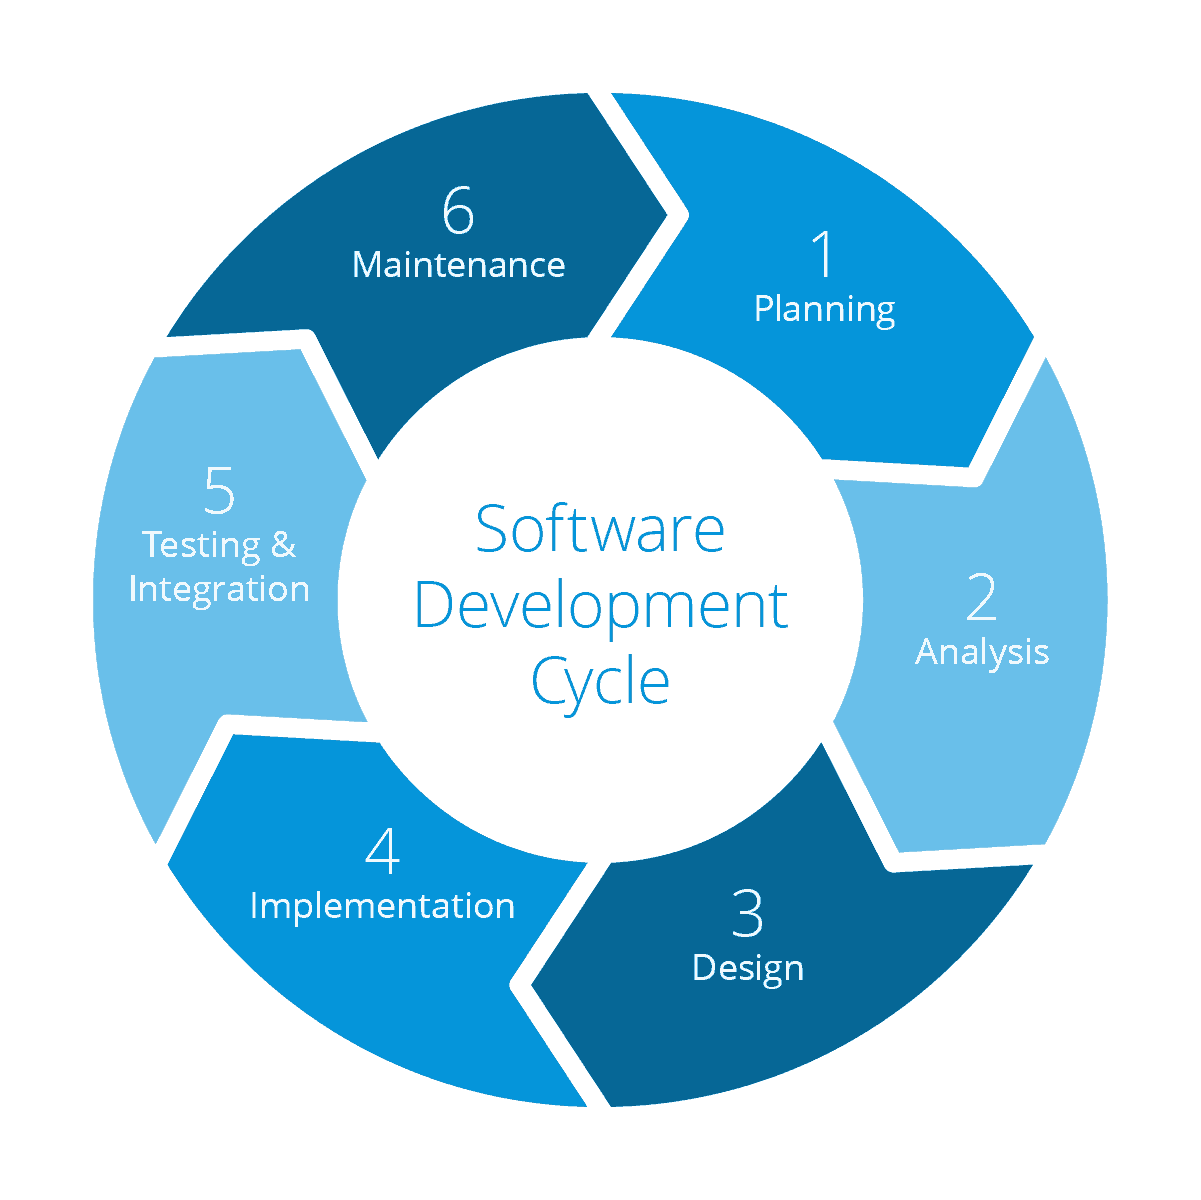
\includegraphics[width=0.3\textwidth]{img/agile.png}
     \caption{Agile Methodology}
    \label{fig:Agile}
\end{figure}

The project management in general is important as it helps to achieve objectives more efficiently and reduce the probability of failure.  It also helped us to organize and prioritize our work.

Even though it was quite tempting to start writing the code straight away before doing that we set up the scope of our project.
We tried to collect user stories or requirements in order to write a prioritized list of work that needs to be done -  Product Backlog. These are the desired functionality that an application should have. Next, the work was divided into small portions in order to minimize the amount of up-front planning and design. 

At the planning stage Jose also drew up the architecture design of our project.
As well at this stage we agreed on technologies and languages that we were going to use. 

Throughout the entire project we tried to meet every week together with our supervisor in order to define the scope of work that needs to be done over the next 7 days. Consequently, our sprints were a week long. At each iteration we tried to add more functionality and reduce the amount of bugs.
 
I think from the very beginning it was clear that Agile software development style Fig.~\ref{fig:Agile} best matches our needs.
The advantages of using Agile over traditional waterfall model or others are numerous. It advocates iterative approach and continuous improvement. Although, it implies a lot of planning, it is also adaptive to changes. It acknowledges that requirements can evolve and change over time.

\subsection{Project Management Tool}
\indent
\indent
As most of the project management tools like Jira or Wrike have only free demo versions for a limited amount of time and our project was a year long, we decided to use github project board. It is free, has all of the functionality a project management tool has and it is very convenient as everything is located in one place.

\subsection{Version Control Tool}
\indent
\indent
Even a small software project cannot do without a version control manager.

The question whether to use GitHub Fig.~\ref{fig:GitHub} or any other tool did not even arise as we used it for most of our college and personal projects and were already familiar with it.
GitHub is a version control tool that provides hosting for software development version control using Git.
It tracks all the changes to documents and files, has tools for basic task management and has excellent documentation. Last but not least it is used by the majority of software companies.

\begin{figure}[ht]
	\centering
	
\includegraphics[width=0.3\textwidth]{img/github.png}
	\caption{GitHub}
	\label{fig:GitHub}
\end{figure}

In our project we tried to create a new branch for every new feature. As soon as the code was written and tested the branch could be merged into master. This approach helped to isolate development work without affecting other branches in the repository (not to mess the master branch and each others code).

As already mentioned in the previous section it was also used as a project management tool.

\subsection{Testing}
\indent
\indent
Testing is an significant part of a development process especially if you are using agile methodology.
In order to test UI manual testing was used, which is also known as a Black box testing (a method of software testing that examines the functionality of an application without peering into its internal structures or workings).
